% Intended LaTeX compiler: pdflatex
\documentclass[10pt,a4paper,UTF8]{article}
\usepackage{zclorg}
\author{emacsun}
\date{}
\title{Thinking in Java chapter6 笔记和习题}
\hypersetup{
 pdfauthor={emacsun},
 pdftitle={Thinking in Java chapter6 笔记和习题},
 pdfkeywords={},
 pdfsubject={},
 pdfcreator={Emacs 25.0.50.1 (Org mode 9.0.5)}, 
 pdflang={English}}
\begin{document}

\maketitle
\tableofcontents
\titlepic{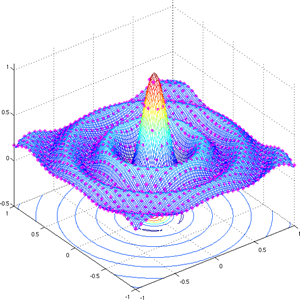
\includegraphics[scale=0.25]{../../img/sinc.PNG}}

\section{简介}
\label{sec:org439b762}
\textbf{Initialization and Cleanup} 这一章首先讲述类初始化的一些操作,顺带初始化操作阐述了方法重载。然后讲述了Java的Garbage Collector机制。其中关于 \texttt{static} 初始化的例子最为令人印象深刻,我把那个“橱柜”的代码做了逐行解析,学完之后感觉非常顺畅。

\section{默认的 \texttt{constructor} 和带参数的 \texttt{constructor}}
\label{sec:org273bd62}


首先默认的 \texttt{constructor} ,看代码:
\begin{verbatim}
import java.util.*;
import static net.mindview.util.Print.*;
class Rock{
    Rock(){
        System.out.println("Rock");
    }
}
public class SimpleConstructor
{
    public static void main(String args[])
    {
        for (int i=0; i < 10 ;i++) {
            new Rock();
        }
    }
}
\end{verbatim}

注意:  \texttt{constructor} 是一个函数,其名称和 \texttt{class} 的名称必须相同(没有为什么,这是规定)。但是没有说明这个函数可不可以携带参数,实际上是可以的, 继续看代码:
\begin{verbatim}
import java.util.*;
import static net.mindview.util.Print.*;
class Rock{
    Rock(int i){
        System.out.print("Rock" + i);
    }
}
public class SimpleConstructor2
{
    public static void main(String args[])
    {
        for (int i=0; i < 10 ;i++) {
            new Rock(i);
        }
    }
}
\end{verbatim}
这段代码的输出是:
\begin{verbatim}
Rock 0 Rock 1 Rock 2 Rock 3 Rock 4 Rock 5 Rock 6 Rock 7 Rock 8 Rock 9
\end{verbatim}
注意在这段代码中使用了 \texttt{print} 而不是 \texttt{println} . \texttt{print} 输出默认不带回车; \texttt{println} 输出默认带回车。

\texttt{constructor} 函数没有返回值,注意这里的没有返回值和 \texttt{void} 函数是两回事。

\texttt{String} 对象初始化值是 \texttt{null}, 看代码:
\begin{verbatim}
import java.util.*;
import static net.mindview.util.Print.*;
class Rock{
    String str;
}
public class Exercise0601
{
    public static void main(String args[])
    {
        Rock rcok = new Rock();
        print("" + rcok.str);
    }
}
\end{verbatim}

其输出为
\begin{verbatim}
null
\end{verbatim}

\section{从 \texttt{constructor} 的定义引入函数重载}
\label{sec:org382d7f0}


作者从 \texttt{constructor} 过度到另一个知识点 \texttt{overload} , 平滑自然。对于重载,值得注意的是 \texttt{primitive} 类型的重载。 看代码:
\begin{verbatim}
import static net.mindview.util.Print.*;
public class PrimitiveOverloading{
    void f1(char x){printnb("f1(char) ");}
    void f1(byte x){printnb("f1(byte) ");}
    void f1(short x){printnb("f1(short) ");}
    void f1(int x){printnb("f1(int) ");}
    void f1(long x){printnb("f1(long) ");}
    void f1(float x){printnb("f1(float) ");}
    void f1(double x){printnb("f1(double) ");}

    void f2(byte x){printnb("f2(byte) ");}
    void f2(short x){printnb("f2(short) ");}
    void f2(int x){printnb("f2(int) ");}
    void f2(long x){printnb("f2(long) ");}
    void f2(float x){printnb("f2(float) ");}
    void f2(double x){printnb("f2(double) ");}

    void f3(short x){printnb("f3(short) ");}
    void f3(int x){printnb("f3(int) ");}
    void f3(long x){printnb("f3(long) ");}
    void f3(float x){printnb("f3(float) ");}
    void f3(double x){printnb("f3(double) ");}

    void f4(int x){printnb("f4(int) ");}
    void f4(long x){printnb("f4(long) ");}
    void f4(float x){printnb("f4(float) ");}
    void f4(double x){printnb("f4(double) ");}

    void f5(long x){printnb("f5(long) ");}
    void f5(float x){printnb("f5(float) ");}
    void f5(double x){printnb("f5(double) ");}

    void f6(float x){printnb("f6(float) ");}
    void f6(double x){printnb("f6(double) ");}

    void f7(double x){printnb("f7(double) ");}

    void testConstVal(){
        printnb("5: ");
        f1(5);f2(5);f3(5);f4(5);f5(5);f6(5);f7(5);print();
    }

    void testChar(){
        char x = 'x';
        printnb("char: ");
        f1(x);f2(x);f3(x);f4(x);f5(x);f6(x);f7(x);print();
    }

    void testByte(){
        byte x = 0;
        printnb("byte: ");
        f1(x);f2(x);f3(x);f4(x);f5(x);f6(x);f7(x);print();
    }

    void testShort(){
        short x = 0;
        printnb("short: ");
        f1(x);f2(x);f3(x);f4(x);f5(x);f6(x);f7(x);print();
    }

    void testInt(){
        int x = 0;
        printnb("int: ");
        f1(x);f2(x);f3(x);f4(x);f5(x);f6(x);f7(x);print();
    }

    void testLong(){
        long x = 0;
        printnb("long: ");
        f1(x);f2(x);f3(x);f4(x);f5(x);f6(x);f7(x);print();
    }

    void testFloat(){
        float x = 0;
        printnb("float: ");
        f1(x);f2(x);f3(x);f4(x);f5(x);f6(x);f7(x);print();
    }

    void testDouble(){
        double x = 0;
        printnb("double: ");
        f1(x);f2(x);f3(x);f4(x);f5(x);f6(x);f7(x);print();
    }

    public static void main(String[] args){
        PrimitiveOverloading p = new PrimitiveOverloading();
        p.testConstVal();
        p.testChar();
        p.testByte();
        p.testShort();
        p.testInt();
        p.testLong();
        p.testFloat();
        p.testDouble();
    }
}
\end{verbatim}
这段代码的输出是:
\begin{verbatim}
5: f1(int) f2(int) f3(int) f4(int) f5(long) f6(float) f7(double) 
char: f1(char) f2(int) f3(int) f4(int) f5(long) f6(float) f7(double) 
byte: f1(byte) f2(byte) f3(short) f4(int) f5(long) f6(float) f7(double) 
short: f1(short) f2(short) f3(short) f4(int) f5(long) f6(float) f7(double) 
int: f1(int) f2(int) f3(int) f4(int) f5(long) f6(float) f7(double) 
long: f1(long) f2(long) f3(long) f4(long) f5(long) f6(float) f7(double) 
float: f1(float) f2(float) f3(float) f4(float) f5(float) f6(float) f7(double) 
double: f1(double) f2(double) f3(double) f4(double) f5(double) f6(double) f7(double)
\end{verbatim}
\section{默认的 \texttt{constructor}}
\label{sec:org5b4ca03}


默认的 \texttt{constructor} 是没有参数的。如果定义类时没有指定构造函数,那么编译器会生成一个默认的构造函数。如果在定义类时指定了构造函数,那么在创建该类的对象时就需要指定该对象实用的构造函数,而不能使用默认构造函数,否则就会报错。看代码:
\lstset{language=java,label= ,caption= ,captionpos=b,firstnumber=1,numbers=left}
\begin{lstlisting}
class Bird{
    Bird(int i){}
    Bird(double d){}
}
public class NoSynthesis{
    public static void main(String[] args){
        Bird b2 = new Bird(1);
        Bird b3 = new Bird(1.0);
        Bird b4 = new Bird();
    }
}
\end{lstlisting}
这个代码会报错:
\begin{verbatim}
error: no suitable constructor found for Bird(no arguments)
        Bird b4 = new Bird();
                  ^
    constructor Bird.Bird(int) is not applicable
      (actual and formal argument lists differ in length)
    constructor Bird.Bird(double) is not applicable
      (actual and formal argument lists differ in length)
1 error
\end{verbatim}

编译器会认为没有无参数的构造函数定义。对代码进行修改:
\lstset{language=java,label= ,caption= ,captionpos=b,firstnumber=1,numbers=left}
\begin{lstlisting}
class Bird{
    Bird(int i){}
    Bird(double d){}
}
public class NoSynthesis{
    public static void main(String[] args){
        Bird b2 = new Bird(1);
        Bird b3 = new Bird(1.0);
    }
}
\end{lstlisting}
就没有报错。但是,看代码:
\lstset{language=java,label= ,caption= ,captionpos=b,firstnumber=1,numbers=left}
\begin{lstlisting}
class Bird{
    Bird(int i){}
    Bird(double d){}
}
public class NoSynthesis{
    public static void main(String[] args){
        Bird b2 = new Bird(1);
        Bird b3 = new Bird(1.0);
        Bird b4;
    }
}
\end{lstlisting}
这个代码也没有报错,但是我不知道 \texttt{b4} 调用了那个构造函数。为了确认一下,对代码做如下修改:
\lstset{language=java,label= ,caption= ,captionpos=b,firstnumber=1,numbers=left}
\begin{lstlisting}
class Bird{
    Bird(int i){
        System.out.println("with int i");
    }
    Bird(double d){
        System.out.println("with double d");
    }
}
public class NoSynthesis{
    public static void main(String[] args){
        Bird b2 = new Bird(1);
        Bird b3 = new Bird(1.0);
        Bird b4;
    }
}
\end{lstlisting}

输出为:
\begin{verbatim}
with int i
with double d
\end{verbatim}
可见 \texttt{Bird b4} 没有调用给出的两个构造函数,而是用的默认的构造函数。
\section{\texttt{this} 的作用}
\label{sec:orgf2d989d}


简而言之, \texttt{this} 用来代表当前的对象。在使用的过程中,你完全可以用 \texttt{this} 来替代当前的对象。但是 \texttt{this} 的实用也会有一些限制,比如只能在 \texttt{non-static} 的方法中使用。但是在一个类的多个方法中不需要显示的使用 \texttt{this} 来指示当前类。

\texttt{this} 的一个经常用到的地方是 \texttt{return} 语句返回一个对象。看代码:
\lstset{language=java,label= ,caption= ,captionpos=b,firstnumber=1,numbers=left}
\begin{lstlisting}
public class Leaf{
    int i=0;
    Leaf increament(){
        i++;
        return this;
    }
    void print(){
        System.out.println(" i = " + i);
    }
    public static void main(String[] args){
        Leaf x = new Leaf();
        x.increament().increament().print();
    }
}
\end{lstlisting}
结果输出为:
\begin{verbatim}
i = 2
\end{verbatim}
\texttt{this} 也可以用来把当前的对象传递给另外的方法,看代码:
\lstset{language=java,label= ,caption= ,captionpos=b,firstnumber=1,numbers=left}
\begin{lstlisting}
class Person{
    public void eat(Apple apple){
        Apple peeled = apple.getPeeled();
        System.out.println("Yummy");
    }
}

class Peeler{
    static Apple peel(Apple apple){
        //...remove peel
        return apple;
    }
}

class Apple{
    Apple getPeeled(){return Peeler.peel(this);}
}

public class PassingThis{
    public static void main(String[] args){
        new Person().eat(new Apple());
    }
}
\end{lstlisting}
\texttt{this} 还可以用来从一个 \texttt{constructor} 中调用另一个 \texttt{constructor} 。这一用途有两点需要注意:
\begin{enumerate}
\item 你不能在一个 \texttt{constructor} 中调用两次 \texttt{this} 初始化函数。
\item 在一个 \texttt{constructor} 中,如果要使用 \texttt{this} ,第一行有效代码就应该是使用 \texttt{this} 的代码。
\end{enumerate}


\section{理解 \texttt{static}}
\label{sec:org08c2f90}


有了 \texttt{this} 我们现在可以更深刻的理解 \texttt{static} 。我们可以从 \texttt{non-static} 函数里调用 \texttt{static} 函数,但是不能从 \texttt{static} 函数里调用 \texttt{non-static} 函数。为什么? 因为在 \texttt{static} 函数里没有对象的概念。 \texttt{static} 函数依赖于 \texttt{class} 的定义存在,而不依赖于对象的存在。所以 \texttt{static} 看起来就像是一个全局方法,不依赖于对象存在。但是 \texttt{Java} 中是没有全局函数的,所以通过 \texttt{static} 可以实现类似的效果。

正是因为 \texttt{static} 的这个特性,人们诟病 \texttt{Java} 的 \texttt{static} 方法不是面向对象的。因为在 \texttt{static} 方法中,无法像一个对象发消息,因为根本没有 \texttt{this} 。因此当你的代码中有很多 \texttt{static} 的时候,你要重新审视一下你的代码结构。但是在很多时候 \texttt{static} 又是一个不得不存在的特性,在以后的章节中就会看到。
\section{\texttt{class} 成员初始化}
\label{sec:org4136063}


\texttt{Java} 中对于 \texttt{class} 的基础类型成员都做了默认初始化。这说明,每一个基础类成员都有一个默认的构造函数,为其赋初值。看代码:
\lstset{language=java,label= ,caption= ,captionpos=b,firstnumber=1,numbers=left}
\begin{lstlisting}
import static net.mindview.util.Print.*;

public class  InitialValues{
    boolean t;
    char c;
    byte b;
    short s;
    int i;
    long l;
    float  f;
    double d;
    InitialValues reference;
    void printInitiaValues(){
        print("Data type         initial values");
        print("boolean           "+t);
        print("char              "+c);
        print("int               "+i);
        print("long              "+l);
        print("float             "+f);
        print("double            "+d);
        print("InitialValues     "+reference);
    }
    public static void main(String[] args){
        InitialValues iv = new InitialValues();
        iv.printInitiaValues();
    }

}
\end{lstlisting}
其输出为:
\begin{verbatim}
Data type         initial values
boolean           false
char              [ ]
int               0
long              0
float             0.0
double            0.0
InitialValues     null
\end{verbatim}
\texttt{char} 的初始值是0,打印出来是一个空格。另外需要注意的是:如果在 \texttt{class} 中定义了一个对象而没有为其赋初值,则这个对象的 \texttt{reference} 会被赋值 \texttt{null}
\section{初始化顺序}
\label{sec:org072a7b8}


在 \texttt{Java} 中,类变量的初始化先于类方法调用。什么意思?就是说:在写代码的时候,即便你把类变量的定义放在了构造函数的后面, \texttt{Java} 依然会先初始化这些变量,然后再去调用函数(这个函数通常是构造函数)。看代码:
\lstset{language=C,label= ,caption= ,captionpos=b,firstnumber=1,numbers=left}
\begin{lstlisting}
import static  net.mindview.util.Print.*;
class Window{
    Window(int marker){
        print("Window number: " + marker);
    }
}
class House{
    Window w1 = new Window(1);
    House(){
        print("House()");
        w3 = new Window(33);
    }
    Window w2 = new Window(2);
    void f(){
        print("f()");
    }
    Window w3 = new Window(3);
}
public class OrderOfInitialization
{
    public static void main(String args[])
    {
        House h = new House();
        h.f();
    }
}
\end{lstlisting}
输出为:
\begin{verbatim}
Window number: 1
Window number: 2
Window number: 3
House()
Window number: 33
f()
\end{verbatim}

从代码中我们可以看到, \texttt{House} 的构造函数在 \texttt{w1} 和 \texttt{w2} 之间。但是我们执行 \texttt{House h = new House()} 这一行代码时,初始化的执行顺序是: 
\begin{enumerate}
\item 初始化  \texttt{w1}
\item 初始化 \texttt{w2}
\item 初始化 \texttt{w3}
\item 调用 \texttt{House()} 对 \texttt{w3} 再次初始化。
\end{enumerate}

\section{\texttt{static} 类型的初始化}
\label{sec:orgb9b48a8}


无论创建了多少个对象, \texttt{static} 类型的数据都只占用一份存储。只有 \texttt{class} 的域可以是 \texttt{static} ,一个本地变量不能是 \texttt{static} 类型的。接下来我们通过一个例子来查看 \texttt{static} 是如何初始化的, 看代码:
\lstset{language=C,label= ,caption= ,captionpos=b,firstnumber=1,numbers=left}
\begin{lstlisting}
// specifying initial values in a class definition
import static net.mindview.util.Print.*;

class Bowl{
    Bowl(int marker){
        print("Bowl(" + marker + ")");
    }
    void f1(int marker){
        print("f1(" + marker + ")");
    }
}

class Table{
    static Bowl bowl =new Bowl(1);
    Table(){
        print("Table()");
        bowl2.f1(1);
    }
    void f2(int marker){
        print("f2(" + marker + ")");
    }
    static Bowl bowl2 = new Bowl(2);
}

class Cupboard{
    Bowl bowl3 = new Bowl(3);
    static Bowl bowl4 = new Bowl(4);
    Cupboard(){
        print("Cupboard()");
        bowl4.f1(2);
    }
    void f3(int marker){
        print("f3(" + marker + ")");
    }
    static Bowl bowl5 =new Bowl(5);
}
public class StaticInitialization
{
    public static void main(String args[])
    {
        print("Creating new Cupboard() in main");
        new Cupboard();
        print("Creating new Cupboard() in main");
        new Cupboard();
        table.f2(1);
        cupboard.f3(1);
    }
    static Table table = new Table();
    static Cupboard cupboard = new Cupboard();
}
\end{lstlisting}

这段代码是我目前敲过的最长的 Java代码,其输出也最长,看输出:
\begin{verbatim}
Bowl(1)
Bowl(2)
Table()
f1(1)
Bowl(4)
Bowl(5)
Bowl(3)
Cupboard()
f1(2)
Creating new Cupboard() in main
Bowl(3)
Cupboard()
f1(2)
Creating new Cupboard() in main
Bowl(3)
Cupboard()
f1(2)
f2(1)
f3(1)
\end{verbatim}

让我们来仔细分析一下每一行的输出是怎么来的。通过 \texttt{Bowl} 我们可以知道初始化的顺序。当我们调用 \texttt{main()} 时,首先初始化的是 \texttt{StaticInitialization} 中的 \texttt{static} 成员,然后是 \texttt{non-static} 成员。在这个代码中是先初始化最后两行的 \texttt{table} 和 \texttt{cupboard} 。

在初始化 \texttt{table} 过程中,生成了前四行输出。 具体过程是:先初始化 \texttt{Table} 的 \texttt{bowl1} 和 \texttt{bowl(2)} 然后调用构造函数 \texttt{Table()} 生成第三行第四行输出。

在初始化 \texttt{cupboard} 过程中,生成了接下来的五行输出。具体过程是:先初始化 \texttt{bowl(4)} 和 \texttt{bowl(5)} 然后初始化 \texttt{bowl3} 最后调用 \texttt{Cupboard()} 构造函数。

\texttt{table} 和 \texttt{cupboard} 初始化结束后, 接下来执行第 41 行打印了一句提示,然后执行第42 行,这个时候由于 \texttt{bowl4} 和 \texttt{bowl5} 已经被初始化了,所以只初始化了 \texttt{bowl3} 并调用了 \texttt{Cupboard()} 构造函数。

然后执行第 43 行,同样的只初始化了 \texttt{bowl3} 并调用了 \texttt{Cupboard()} 构造函数。

最后调用 \texttt{table.f2(2)} 和 \texttt{cupboard.f3(1)} 生成最后两行输出。
\section{显示初始化}
\label{sec:org4667218}


在 \texttt{Java} 中可以使用 \texttt{static} 语句初始化(有时候我们叫之中初始化方式为 \texttt{static} 块)。看代码:
\lstset{language=java,label= ,caption= ,captionpos=b,firstnumber=1,numbers=left}
\begin{lstlisting}
public class Spoon{
    static int i;
    static{
        i = 47;
    }
}
\end{lstlisting}
看起来像是一个方法,但是注意这种初始化方法仅仅是一个 \texttt{static} 关键词跟着一个语句块。同其他 \texttt{static} 初始化语句一样,使用 \texttt{static} 块的初始化也仅仅执行一次。看代码:
\lstset{language=C++,label= ,caption= ,captionpos=b,firstnumber=1,numbers=left}
\begin{lstlisting}
class Cup{
  Cup(int marker){
    print("Cup(" + marker + ")");
  }
  void f(int marker){
    print("f(" + marker + ")");
  }
}

class Cups{
  static Cup cup1;
  static Cup cup2;
  static{
    cup1 = new Cup(1);
    cup2 = new Cup(2);
  }
  Cups(){
    print("Cups()"); 
  }
}

public class ExplicitStatic{
  public static void main(String[] args){
    print("Inside main()");
    Cups.cup1.f(99);                           (cupsrun)
  }
  static Cups cups1 = new Cups();              (cupsrun1)
}
\end{lstlisting}

输出为:
\begin{verbatim}
Inside main()
Cup(1)
Cup(2)
f(99)
\end{verbatim}

\texttt{static} 初始化语句在下列任一情况下初始化 \texttt{Cups} :
\begin{enumerate}
\item 第cupsrun 行执行。
\item 第cupsrun 被注释,第cupsrun1 行解注;
\end{enumerate}

在情况1, 我们访问了 \texttt{Cups}  的成员变量,这个时候出发了 \texttt{Cups} 类的初始化;在情况2,我们初始化了对象 \texttt{cups1} 。

当我们把第 cupsrun1行解注,第cupsrun 注释掉之后,输出为:
\begin{verbatim}
Cup(1) 
Cup(2)
Cups()
Inside main()
\end{verbatim}

可以看到在类 \texttt{ExplicitStatic} 中,也是 \texttt{static} 变量先初始化。我们看到 \texttt{Inside main()} 最后输出。说明程序先完成了静态成员 \texttt{cups1} 的初始化之后再调用的 \texttt{main} 函数。

如果我把第 cupsrun1行和第cupsrun 行都解注,则输出:
\begin{verbatim}
Cup(1)
Cup(2)
Cups()
Inside main()
f(99)
\end{verbatim}
可以看出还是 \texttt{static} 变量优先,通过第 cupsrun1行对 \texttt{Cups} 类的静态变量进行了初始化。然后再执行 \texttt{main} 函数。


\begin{problem}
Create a class with a \texttt{static String} field that is initialized at the point of definition, and another one that is initialized by the \texttt{static} block. Add a \texttt{static} method that prints both fields and demonstrates that they are both initialized before they are used.
\end{problem}
\begin{answer}
首先编写代码,如下

\lstset{language=C,label= ,caption= ,captionpos=b,firstnumber=1,numbers=left}
\begin{lstlisting}
import static net.mindview.util.Print.*;

class String1{
    static String str1 = "string in String1";
    String1(){
        print("" + str1);
    }
}
class String2{
    static String str2;
    static{
        str2 = "string in string2";
    }
    String2(){
        print("" + str2);
    }
}

public class Exercise0614{
    public static void main(String[] args){
        print("Inside main()");
        String1 str1 = new String1();
        String2 str2 = new String2();
    }
}
\end{lstlisting}
输出为:
\begin{verbatim}
Inside main()
string in String1
string in string2
\end{verbatim}
之所以按顺序初始化 \texttt{str1} 和 \texttt{str2} ,是因为在 \texttt{Exercise0614} 的类中,这两个变量不是 \texttt{static} ,把这两个类改成 \texttt{static} 的有:
\lstset{language=C,label= ,caption= ,captionpos=b,firstnumber=1,numbers=left}
\begin{lstlisting}
import static net.mindview.util.Print.*;

class String1{
    static String str1 = "string in String1";
    String1(){
        print("" + str1);
    }
}
class String2{
    static String str2;
    static{
        str2 = "string in string2";
    }
    String2(){
        print("" + str2);
    }
}

public class Exercise0614{
    public static void main(String[] args){
        print("Inside main()");
    }
    static String1 str1 = new String1();
    static String2 str2 = new String2();

}
\end{lstlisting}
输出为:
\begin{verbatim}
string in String1
string in string2
Inside main()
\end{verbatim}

然后修改代码,为其添加静态函数(静态函数可以在不定义对象的时候调用,而我们调用静态函数的同时,对这个静态函数所属的类初始化,主要是初始化其 \texttt{static} 变量)。
\lstset{language=C,label= ,caption= ,captionpos=b,firstnumber=1,numbers=left}
\begin{lstlisting}
import static net.mindview.util.Print.*;

class String1{
    static String str1 = "string in String1";
    String1(){
        print("construct 1" + str1);
    }
    static void f1(){
        print("static method" + str1);
    }
}
class String2{
    static String str2;
    static{
        str2 = "string in string2";
    }
    String2(){
        print("constructor 2" + str2);
    }
    static void f2(){
        print("static method" + str2);
    }
}

public class Exercise0614{
    public static void main(String[] args){
        print("Inside main()");
        String2.f2();
        String1.f1();
    }
    static String2 str2 = new String2();
}
\end{lstlisting}
输出为:
\begin{verbatim}
constructor 2string in string2
Inside main()
static methodstring in string2
static methodstring in String1
\end{verbatim}
\end{answer}
\section{非静态实例初始化}
\label{sec:org051c087}


对于非静态变量, java提供了类似于 \texttt{static} 块的初始化方式。看代码:

\lstset{language=C,label= ,caption= ,captionpos=b,firstnumber=1,numbers=left}
\begin{lstlisting}
import static net.mindview.util.Print.*;

class Mug{
    Mug(int marker){
        print("Mug("  + marker +")");
    }
    void f(int marker){
        print("f(" + marker + ")");
    }
}
public class Mugs{
    Mug mug1;
    Mug mug2;
    {
        mug1 = new Mug(1);
        mug2 = new Mug(2);
        print("mug1 & mug2 initialized");
    }
    Mugs(){
        print("Mugs()");
    }
    Mugs(int i){
        print("Mugs(int)");
    }
    public static void main(String[] args){
        print("Inside main()");
        new Mugs();
        print("new Mugs() completed");
        new Mugs(1);
        print("new Mugs(1) completed");
    }
}
\end{lstlisting}
输出为:
\begin{verbatim}
Inside main()
Mug(1)
Mug(2)
mug1 & mug2 initialized
Mugs()
new Mugs() completed
Mug(1)
Mug(2)
mug1 & mug2 initialized
Mugs(int)
new Mugs(1) completed
\end{verbatim}
从这个输出可以看出,实例可以按照顺序初始化,没有像 \texttt{static} 一样执行顺序和代码出现顺序不一样的情况。
\section{数组初始化}
\label{sec:org8574756}


数组是一些相同类型元素的集合。这些元素可以是基础类型也可以是某个类(这么说可能有些不严谨,基础类型也是类,在Java中一切都是类。)。

定义一个整型数组可以使用 \texttt{int[] a1;} 也可以用 \texttt{int a1[]} 。在 \texttt{Java} 中,数组的初始化可以通过大括号实现,也可以不初始化。 \texttt{Java} 中,数组名的赋值,复制的是引用。看代码:
\lstset{language=C,label= ,caption= ,captionpos=b,firstnumber=1,numbers=left}
\begin{lstlisting}
import static net.mindview.util.Print.*;

public class ArrayOfPrimitives{
    public static void main(String[] args){
        int[] a1 = {1,2,3,4,5};
        int[] a2;
        a2 = a1;
        for (int i = 0; i < a1.length; i++) {
            a2[i] = a2[i]*2;
        }
        for (int i = 0; i < a1.length; i++) {
            print("a1[" + i + "]= " + a1[i]);
        }
    }
}
\end{lstlisting}
输出是:
\begin{verbatim}
a1[0]= 2
a1[1]= 4
a1[2]= 6
a1[3]= 8
a1[4]= 10
\end{verbatim}
可以看到执行了 \texttt{a2=a1} 之后, \texttt{a2} 指向的内容和 \texttt{a1} 指向的内容是一样的。 这时候即使对 \texttt{a2} 进行修改, \texttt{a1} 的内容也同时发生了改变。

关于数组越界的问题在 \texttt{C/C++} 和 \texttt{Java} 中有不同的处理方法: \texttt{C/C++} 不会对数组越界进行约束,而 \texttt{Java} 会。在 \texttt{Java} 中,一旦数组越界就会报错。 虽然适时的检查会不会报错是一件很低效的事情,但是为了开发效率, \texttt{Java} 的设计者认为这是值得的。

对于事先不知道长度的数组,需要用 \texttt{new} 来为其分配空间,看代码:

\lstset{language=C,label= ,caption= ,captionpos=b,firstnumber=1,numbers=left}
\begin{lstlisting}
import java.util.*;
import static net.mindview.util.Print.*;

public class ArrayNew{
    public static void main(String[] args){
        int [] a;
        Random rand = new Random(47);
        a = new int[rand.nextInt(20)];
        print("length of a = " + a.length );
        print(Arrays.toString(a));
    }
}
\end{lstlisting}
输出为:
\begin{verbatim}
length of a = 18
[0, 0, 0, 0, 0, 0, 0, 0, 0, 0, 0, 0, 0, 0, 0, 0, 0, 0]
\end{verbatim}

之前创建了 \texttt{primitive} 的数组。现在创建对象数组,当创建对象数组时,数组元素是对象的索引。现在考虑创建 \texttt{Integer} 数组。(回忆一下 \texttt{Integer} 是类不是primitive类型。 基础类型和类的区别是,基础类型保存在栈上,而对象保存在堆上。)

\lstset{language=C,label= ,caption= ,captionpos=b,firstnumber=1,numbers=left}
\begin{lstlisting}
import java.util.*;
import static net.mindview.util.Print.*;

public class ArrayClassObj{
    public static void main(String[] args){
        Random rand = new Random(47);
        Integer[] a = new Integer[rand.nextInt(10)];
        print(Arrays.toString(a));
        print("length of a = " + a.length);
        for (int i = 0; i < a.length; i++) {
            a[i] = rand.nextInt(500);
        }
        print(Arrays.toString(a));
    }
}
\end{lstlisting}
输出是:
\begin{verbatim}
[null, null, null, null, null, null, null, null]
length of a = 8
[55, 193, 361, 461, 429, 368, 200, 22]
\end{verbatim}
从代码可以看出,没有初始化之前打印输出的都是 \texttt{null} 而不是像基础类型那样初始化为 \texttt{0} ,只有初始化之后才会有数据打印。在创建对象数组时,即使使用 \texttt{new} 也没有初始化这个数组,必须一个一个来。

对于对象数组也可以用大括号进行初始化,看代码:
\lstset{language=C,label= ,caption= ,captionpos=b,firstnumber=1,numbers=left}
\begin{lstlisting}
import java.util.*;

public class ArrayInit{
    public static void main(String[] args){
        Integer[] a = {
            new Integer(1),
            new Integer(2),
            3,
        };
        Integer[] b = new Integer[]{
            new Integer(1),
            new Integer(2),
            3,
        };
        System.out.println(Arrays.toString(a));
        System.out.println(Arrays.toString(b));
    }
}
\end{lstlisting}
输出为:
\begin{verbatim}
[1, 2, 3]
[1, 2, 3]
\end{verbatim}

注意初始化对象数组时,最后一个元素后面的逗号。使用这个逗号写出的代码便于维护,尤其是维护长数组。可以用这种初始化方法传递变长参数。看代码:

\lstset{language=C,label= ,caption= ,captionpos=b,firstnumber=1,numbers=left}
\begin{lstlisting}
class A{}

public class VarArgs{
    static void printArray(Object[] args){
        for (Object obj: args)
            System.out.print(obj + " ");
        System.out.println();
    }
    public static void main(String[] args){
        printArray(new Object[]{
                new Integer(47), new Float(3.14),new Double(11.11),
            });
        printArray(new Object[]{"one","two","three"});
        printArray(new Object[]{new A(),new A(),new A()});
    }
}
\end{lstlisting}
输出是:
\begin{verbatim}
47 3.14 11.11 
one two three 
A@15db9742 A@6d06d69c A@7852e922
\end{verbatim}
上面代码的 \texttt{Object} 共有的根类,关于这个类,我们后面还会学到更多。因为所有类都是从 \texttt{Object} 继承而来,所以可以把 \texttt{Object} 数组传入一个方法。

另外我们还可以看到, \texttt{print} 函数接收一个 \texttt{Object} 的数组,然后用 \texttt{foreach} 的循环语法打印每个 \texttt{Object} 数组中 \texttt{reference} 对应的内容。打印标准的 \texttt{Java} 库类输出具有较强的可读性(看输出的前两行),打印自定义的类的输出(输出的第三行)就有点不知所云。不过从输出的第三行可以看出打印自定义类,其输出具有固定的格式,都是类名跟上 \texttt{@} 然后是一串十六进制数(以后我们会了解到,这串十六进制数是对象地址)。

上面的这段代码在 Java SE5之前比较常见,但是自从 Java SE5之后,就有更方便的写法了:可以像  \texttt{printArray()} 那样打印数组(我现在写这个笔记的时候用的是SE8,所以浪费了一段时间学习了一个历史技术。)。

看代码:
\lstset{language=C,label= ,caption= ,captionpos=b,firstnumber=1,numbers=left}
\begin{lstlisting}
public class NewVarArgs{
    static void printArray(Object... args){
        for (Object obj : args) {
            System.out.print(obj + " ");
        }
        System.out.println();
    }
    public static void main(String[] args){
        printArray(new Integer(47),new Float(3.14),new Double(11.11));
        printArray(47,3.14F,11.11); 
        printArray("one","two","three");
        printArray(new A(),new A(),new A());
        printArray((Object[])new Integer[]{1,2,3,4});                       (NewVarArgsline2)
        printArray();//Empth list is also OK;
    }
}
\end{lstlisting}
输出为:
\begin{verbatim}
47 3.14 11.11 
47 3.14 11.11 
one two three 
A@15db9742 A@6d06d69c A@7852e922 
1 2 3 4
\end{verbatim}

开心的服下这颗语法糖。

当你使用 \texttt{varargs} 时,不在需要写明数组信息,编译器会自动帮你填写。编译器会给 \texttt{print()} 函数一个 \texttt{array} 。但是注意这里不仅仅是从一个元素列表到一个数组的转换。注意代码中第NewVarArgsline2 行,我们可以看到一个 \texttt{Integer} 数组转换成了一个 \texttt{Object} 数组。 \emph{在编译过程中,编译器看到这是一个数组,并不会做转换}  (对这句话我还没有深刻的理解,需要以后回头看)。

最后一行代码告诉我们,可以对一个 \texttt{vararg} 的列表传送零个参数。这个语法很有用,尤其是当函数的尾随参数个数可变时。关于尾随参数,看代码:
\lstset{language=C,label= ,caption= ,captionpos=b,firstnumber=1,numbers=left}
\begin{lstlisting}
public class OptionalTrailingArguments{
    static void f(int required, String... trailing){
        System.out.print("required: " + required + " ");

        for(String s: trailing)
            System.out.print(s + " ");
        System.out.println();
    }
    public static void main(String[] args){
        f(1,"one");
        f(2,"two","three");
        f(0);
    }
}
\end{lstlisting}
输出为:
\begin{verbatim}
required: 1 one 
required: 2 two three 
required: 0
\end{verbatim}

从上面代码还可以看出,可以使用除了 \texttt{Object} 之外的类型作为 \texttt{varargs} 的类型(在这里例子中,我们实用的是 \texttt{String} )。事实上,可以使用任何类型作为可变参数类型。看代码:
\lstset{language=C,label= ,caption= ,captionpos=b,firstnumber=1,numbers=left}
\begin{lstlisting}
public class VarargType{
    static void f(Character... args){
        System.out.print(args.getClass());
        System.out.println(" length " + args.length);
    }
    static void g(int ... args){
        System.out.print(args.getClass());
        System.out.println(" length " + args.length);
    }
    public static void main(String[] args){
        f('a');
        f();
        g(1);
        g();
        System.out.println("int []: " + new int[0].getClass());
    }
}
\end{lstlisting}
输出为:
\begin{verbatim}
class [Ljava.lang.Character; length 1
class [Ljava.lang.Character; length 0
class [I length 1
class [I length 0
int []: class [I
\end{verbatim}

从上面的代码可以看出,可以使用 \texttt{Character} 数组作为可变参数类型,也可以使用 \texttt{int} 这种基础类型作为可变参数类型。 \texttt{getClass()} 函数是 \texttt{Object} 的内置函数。 
\end{document}
